\chapter{三维光场人脸视频动态光照编辑}
在前一章节中，围绕三维光场静态人像光照编辑问题，本文构建了基于单帧视觉质量优化的重光照生成框架，实现了在多视角图像条件下兼具较高真实感与光照可控性的三维光场人像重光照效果。然而在实际应用中，三维光场内容往往以视频序列形式呈现，仅依赖单帧优化难以满足动态显示需求。当静态光照编辑方法直接扩展至视频序列时，时间维度上易出现亮度闪烁、高光抖动及阴影跳变等问题；同时，光场数据由多视角图像共同构成，若各视角之间缺乏统一约束，还会在空间维度引发光照响应不一致，从而削弱三维立体感与观看沉浸感。

针对上述问题，本章面向三维光场人像视频动态光照编辑场景，在第三章关键信息驱动的三维光场静态人脸光照编辑的基础上，从时间一致性与多视角空间一致性两个关键维度出发，提出一种联合优化框架，以实现跨帧光照连续性与跨视角光照统一性的协同提升。与传统仅关注二维视频稳定性的重光照方法不同，本文方法将光场数据的“时间—空间双维一致性”作为核心约束目标，在保证光照编辑可控性的同时兼顾几何结构稳定与视差连续性需求，从而更契合三维光场显示系统的真实观看特性。

\begin{figure}[H]
  \centering
  %\vspace{1 cm} % 使用该指令调整上下间距
  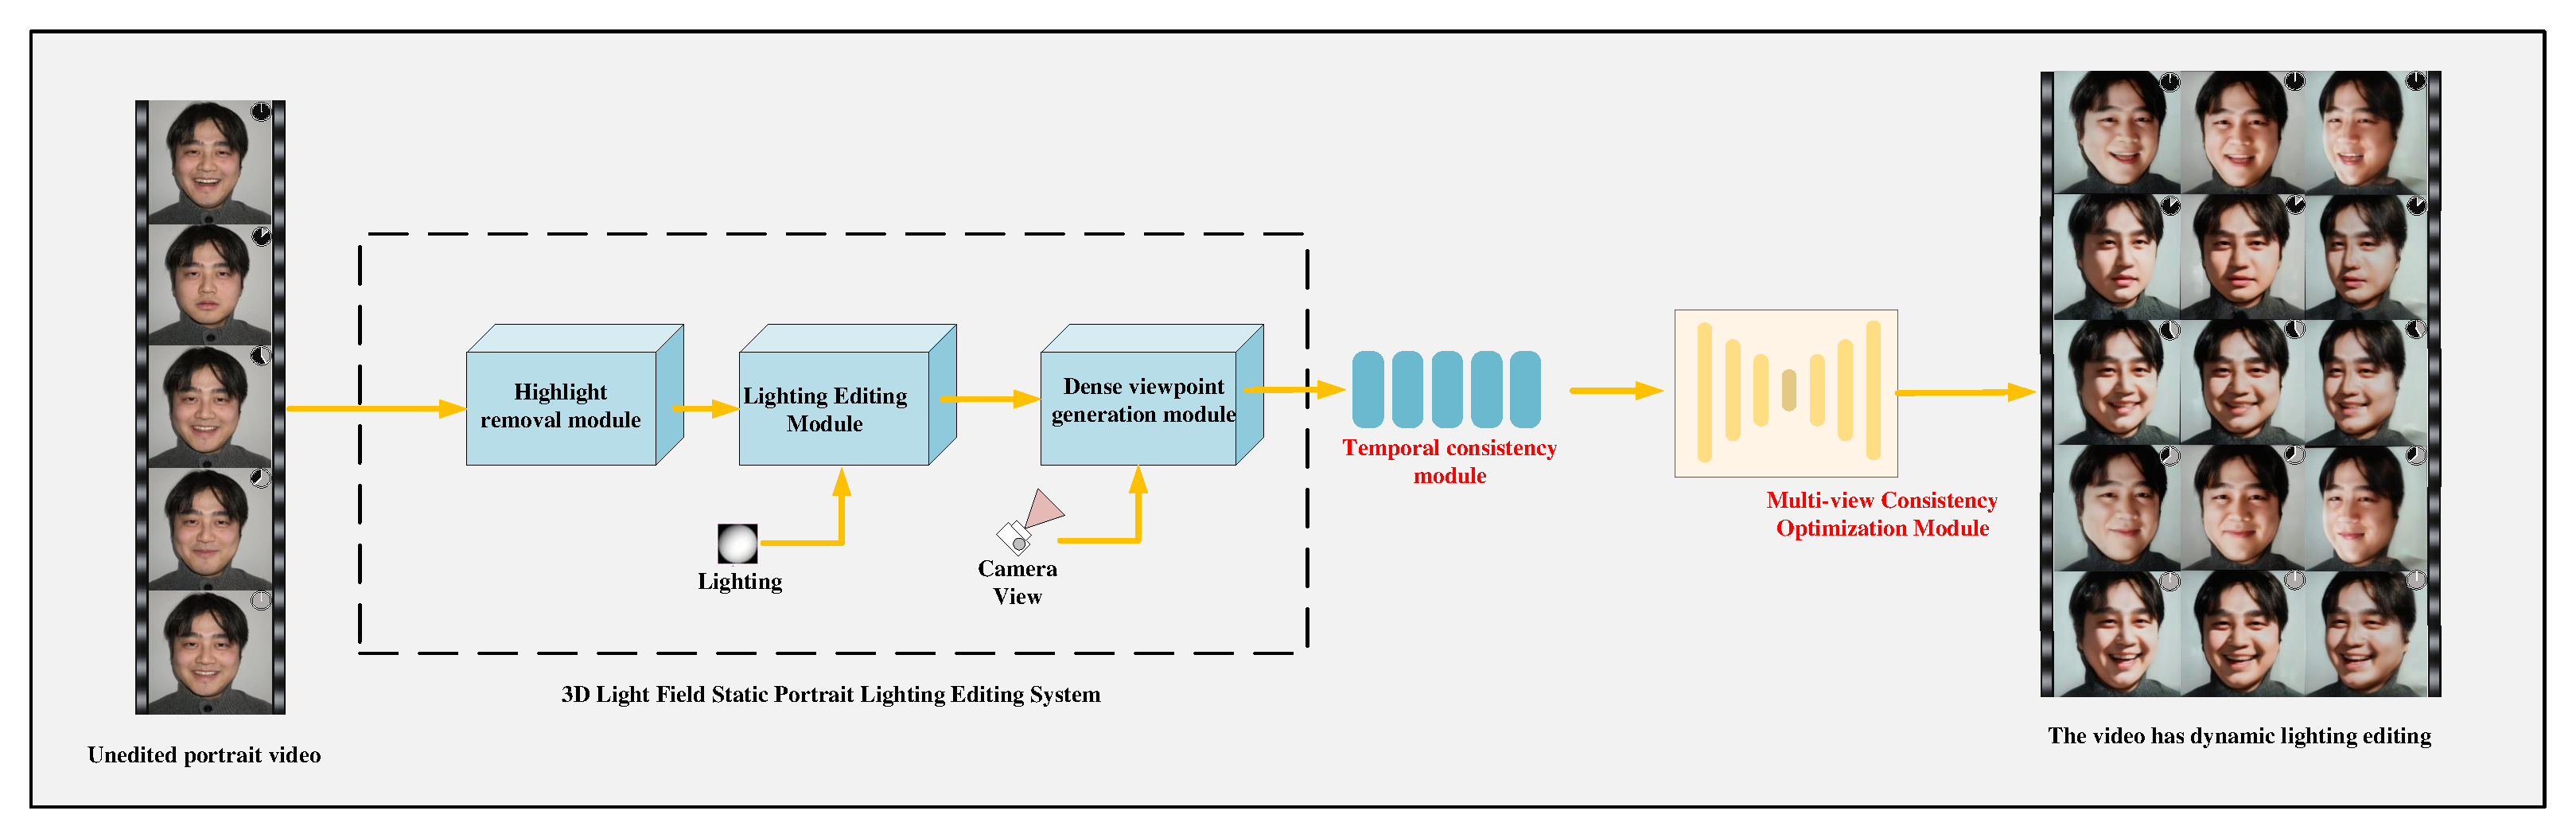
\includegraphics[width=0.9\textwidth,height=5cm]{resources/4p/4-1.pdf}
  % \bicaption{中文标题}{English Caption} % 使用中英文标题
  \caption{总体流程图} % 只使用中文标题
  \label{fig:4-1}
  %\vspace{1 cm} % 使用该指令调整上下间距
\end{figure}
具体流程如图\ref{fig:4-1}所示：在第三章关键信息驱动的三维光场静态人脸光照编辑框架上，新增时序一致性模块与多视角一致性模块，以满足三维光场人像视频动态光照编辑场景下的动态显示需求：

具体而言，本章在第三章关键信息驱动的三维光场静态人脸光照编辑的现有框架上，首先构建基于特征分离的时序一致性优化模块，通过共享编码网络与光流对齐机制，对视频序列中的光照语义分量进行选择性时间约束，在抑制光照闪烁的同时保留表情与姿态的自然变化。随后，引入基于三维几何对齐的多视角一致性优化模块，通过三维表面采样与光照语义加权聚合策略，将多视角光照统一问题转化为三维空间光照估计问题，实现不同观察方向下光照响应的物理一致性表达。最后，通过多组定性与定量实验，从视觉真实感、时间一致性及多视角一致性等多个维度对所提出方法进行系统验证，并进行消融实验进一步分析各关键模块对整体性能的贡献。



\section{基于特征分离与双重约束的时序一致性优化}
在三维光场人像视频光照编辑任务中，除单帧视觉质量外，时间维度的一致性同样是影响最终观感的重要因素。若对视频序列逐帧独立进行光照编辑，即便每一帧在静态观察下均具有较好的视觉效果，在连续播放时仍可能产生明显的亮度闪烁、高光抖动及阴影跳变等现象。这类问题在面部区域尤为突出，容易破坏人像的真实感与沉浸感。因此，在静态光照编辑框架的基础上，本文引入时序一致性优化模块，通过跨帧特征对齐、光照—几何特征分离以及时间残差平滑等多重机制，对视频中光照变化进行显式建模与约束，从而在保证人脸动态自然性的同时显著提升时间维度的稳定性。

与传统视频平滑方法直接对整帧图像或整体特征进行统一约束不同，本文认为在人像光照编辑场景中，不同语义属性在时间维度上具有差异化稳定特性：身份与几何结构在短时间内应保持相对稳定，而光照响应则应在编辑控制下呈现连续变化趋势。若对二者施加同等强度的时间平滑约束，往往会导致表情拖影、嘴部模糊或姿态迟滞等副作用。基于上述问题，本章提出一种特征分离与双重约束的时序一致性策略，在特征空间中仅对光照相关分量进行时间约束，从而在抑制光照闪烁的同时保留面部表情与头部运动的自然变化，具体流程如图\ref{fig:4-2}所示。
\begin{figure}[htbp]
  \centering
  %\vspace{1 cm} % 使用该指令调整上下间距
  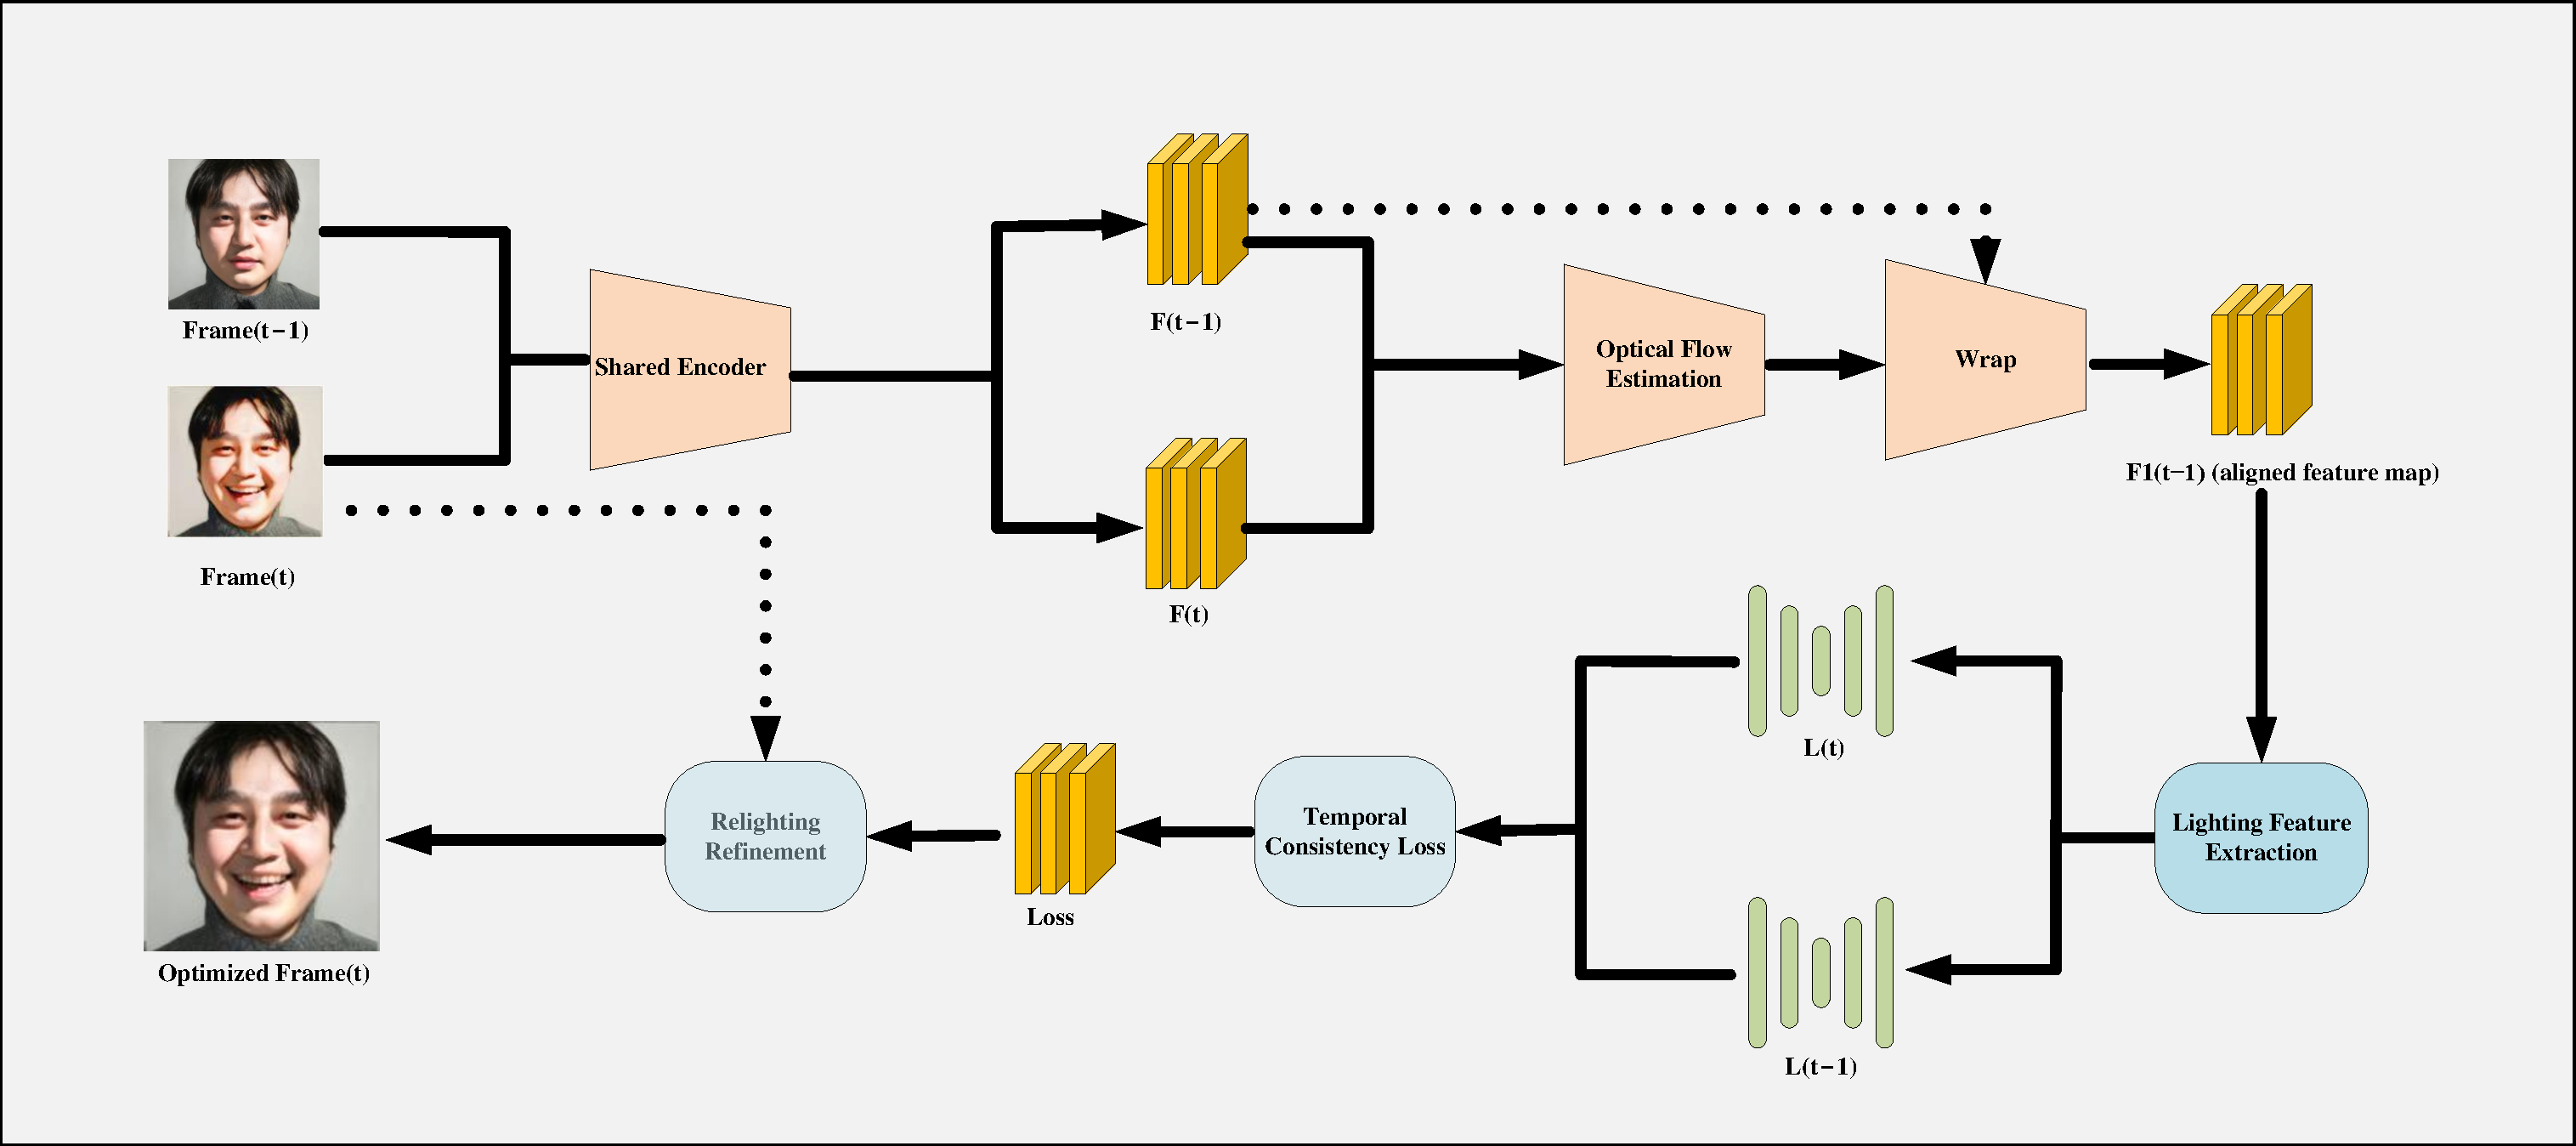
\includegraphics[width=0.9\textwidth,height=6cm]{resources/4p/4-2.pdf}
  % \bicaption{中文标题}{English Caption} % 使用中英文标题
  \caption{时序一致性优化流程图} % 只使用中文标题
  \label{fig:4-2}
  %\vspace{1 cm} % 使用该指令调整上下间距
\end{figure}

设输入视频序列中连续两帧经初始重光照处理后的结果分别为 \(I_{t-1}, I_t\)。

为获得具有时间鲁棒性的高层语义表达，本章引入共享权重卷积编码网络（Shared Encoder）对相邻帧进行特征提取。共享权重设计的核心优势在于保证特征空间分布的一致性，使不同时间帧在嵌入空间中具有可比性，从而避免因网络参数差异引入的伪时间误差。

与双编码器结构相比，共享编码策略不仅降低模型参数规模，同时在训练阶段天然形成跨帧语义对齐约束，有助于提升身份一致性与几何稳定性。这一设计在三维光场人像场景中尤为关键，因为光场显示系统对多视角与多时间维度均存在一致性要求，任何单帧偏移都可能在空间重建中被放大。

设输入视频中连续两帧经初始重光照后的图像分别为：\(I_{t-1}, I_t\)。为获得稳定的语义表达，共享权重卷积编码网络，公式如下：
\begin{equation}
F_{t-1} = E(I_{t-1}), \quad F_t = E(I_t)
\end{equation}

由于相邻帧之间不可避免存在头部微动、表情变化及视角偏移，若直接在特征空间中施加一致性损失，会导致空间错位误差并削弱优化效果。因此本文引入光流估计网络 Warp 预测二维位移向量场，用以描述像素级运动趋势。随后通过双线性采样函数对前一帧特征进行空间变换，实现跨帧特征对齐。该步骤的意义在于：将“时间一致性问题”转化为“空间对齐问题”，从而避免将真实运动误判为光照闪烁。

与直接时间滤波方法相比，光流引导的对齐机制在保持运动真实性方面具有明显优势，能够有效减少嘴部运动模糊与头部轮廓拖影。

光流估计网络可表示为：
\begin{equation}
M_{t-1 \to t} = \phi(F_{t-1}, F_t)
\end{equation}
其中 \(M_{t-1 \to t}\) 为二维位移向量场。随后利用双线性采样函数对前一帧特征进行变换：
\begin{equation}
\tilde{F}_{t-1} = W(F_{t-1}, M_{t-1 \to t})
\end{equation}
为了避免对几何变化过度约束，引入设计光照分量提取网络进行光照特征提取。为避免对几何变化与身份语义产生过度约束，设计光照分量提取网络，将共享编码特征映射至光照响应子空间，仅保留亮度趋势、高光分布与阴影方向等与光照相关的信息。通过语义解耦策略，将“光照一致性”与“几何一致性”在特征层面分离，从而实现选择性时间优化。这一步骤的核心点在于：并非在像素域或整体特征域进行时间约束，而是在语义可控的光照子空间中进行一致性建模。

光照分量提取网络可表示为：
\begin{equation}
L_t = D(F_t), \quad L_{t-1} = D(\tilde{F}_{t-1})
\end{equation}
其中 \(L\) 表示光照响应特征，仅保留亮度趋势、高光分布与阴影方向信息。

在 Temporal Consistency Loss 部分，获得光照语义特征后，在特征空间中采用 L1 距离构建核心时间一致性约束。选择 L1 而非 L2 的原因在于，L1 损失对局部高光区域具有更强鲁棒性，不会因极值像素而产生过度平滑效应，从而保留真实光照变化边界。然而，仅在特征层进行约束仍可能残留像素级闪烁现象，因此进一步引入残差趋势约束。通过计算光照残差并在时间维度上施加平滑损失，使系统不仅在语义层面保持稳定，同时在像素响应层面抑制突变。最终时序一致性损失函数由特征一致性项与残差趋势项加权组成，实现双重时间约束。相关公式如下：

设原始帧为 \(I_t^{orig}\)，则光照残差为：
\begin{equation}
R_t = I_t - I_t^{orig}
\end{equation}

时间平滑损失为：
\begin{equation}
\partial_{TC} = \lambda_1 \delta_{feat} + \lambda_2 \delta_{res}
\end{equation}

最终时序一致性损失函数定义为：
\begin{equation}
\delta_{res} = \left\| R_t - R_{t-1} \right\|_2
\end{equation}

通过双重约束机制，系统既保证光照语义稳定，又抑制像素级跳变。

在获得时间一致的光照特征后，最终通过轻量级卷积细化网络生成优化后的输出图像。该网络主要负责局部细节恢复与颜色校正，其结构设计强调低参数量与高推理效率，以满足视频级处理需求。与直接输出策略相比，引入细化阶段能够有效修正边缘过渡与高光扩散问题，使最终结果在连续播放条件下呈现更加自然平滑的视觉效果。

在获得时序一致特征后，最终通过轻量级卷积网络，生成优化后的图像，公式如下：
\begin{equation}
I_t^{final} = R(I_t, \partial_{TC})
\end{equation}

\section{基于几何对齐与多因子聚合的的多视角一致性优化}
在三维光场人像视频光照编辑任务中，时间维度的一致性保证了视频播放过程中的稳定性，而视角维度的一致性则直接决定空间真实感与立体连续性。光场数据本质上由多个视角图像共同构成，其显示效果依赖于观察者在不同视点间的连续切换体验。若各视角独立进行光照编辑，即便单视角结果具有较高视觉质量，在跨视角观察时仍可能产生亮度不匹配、高光位置漂移以及阴影方向错位等问题，从而破坏三维空间连续性与沉浸式感知效果。

\begin{figure}[htbp]
  \centering
  %\vspace{1 cm} % 使用该指令调整上下间距
  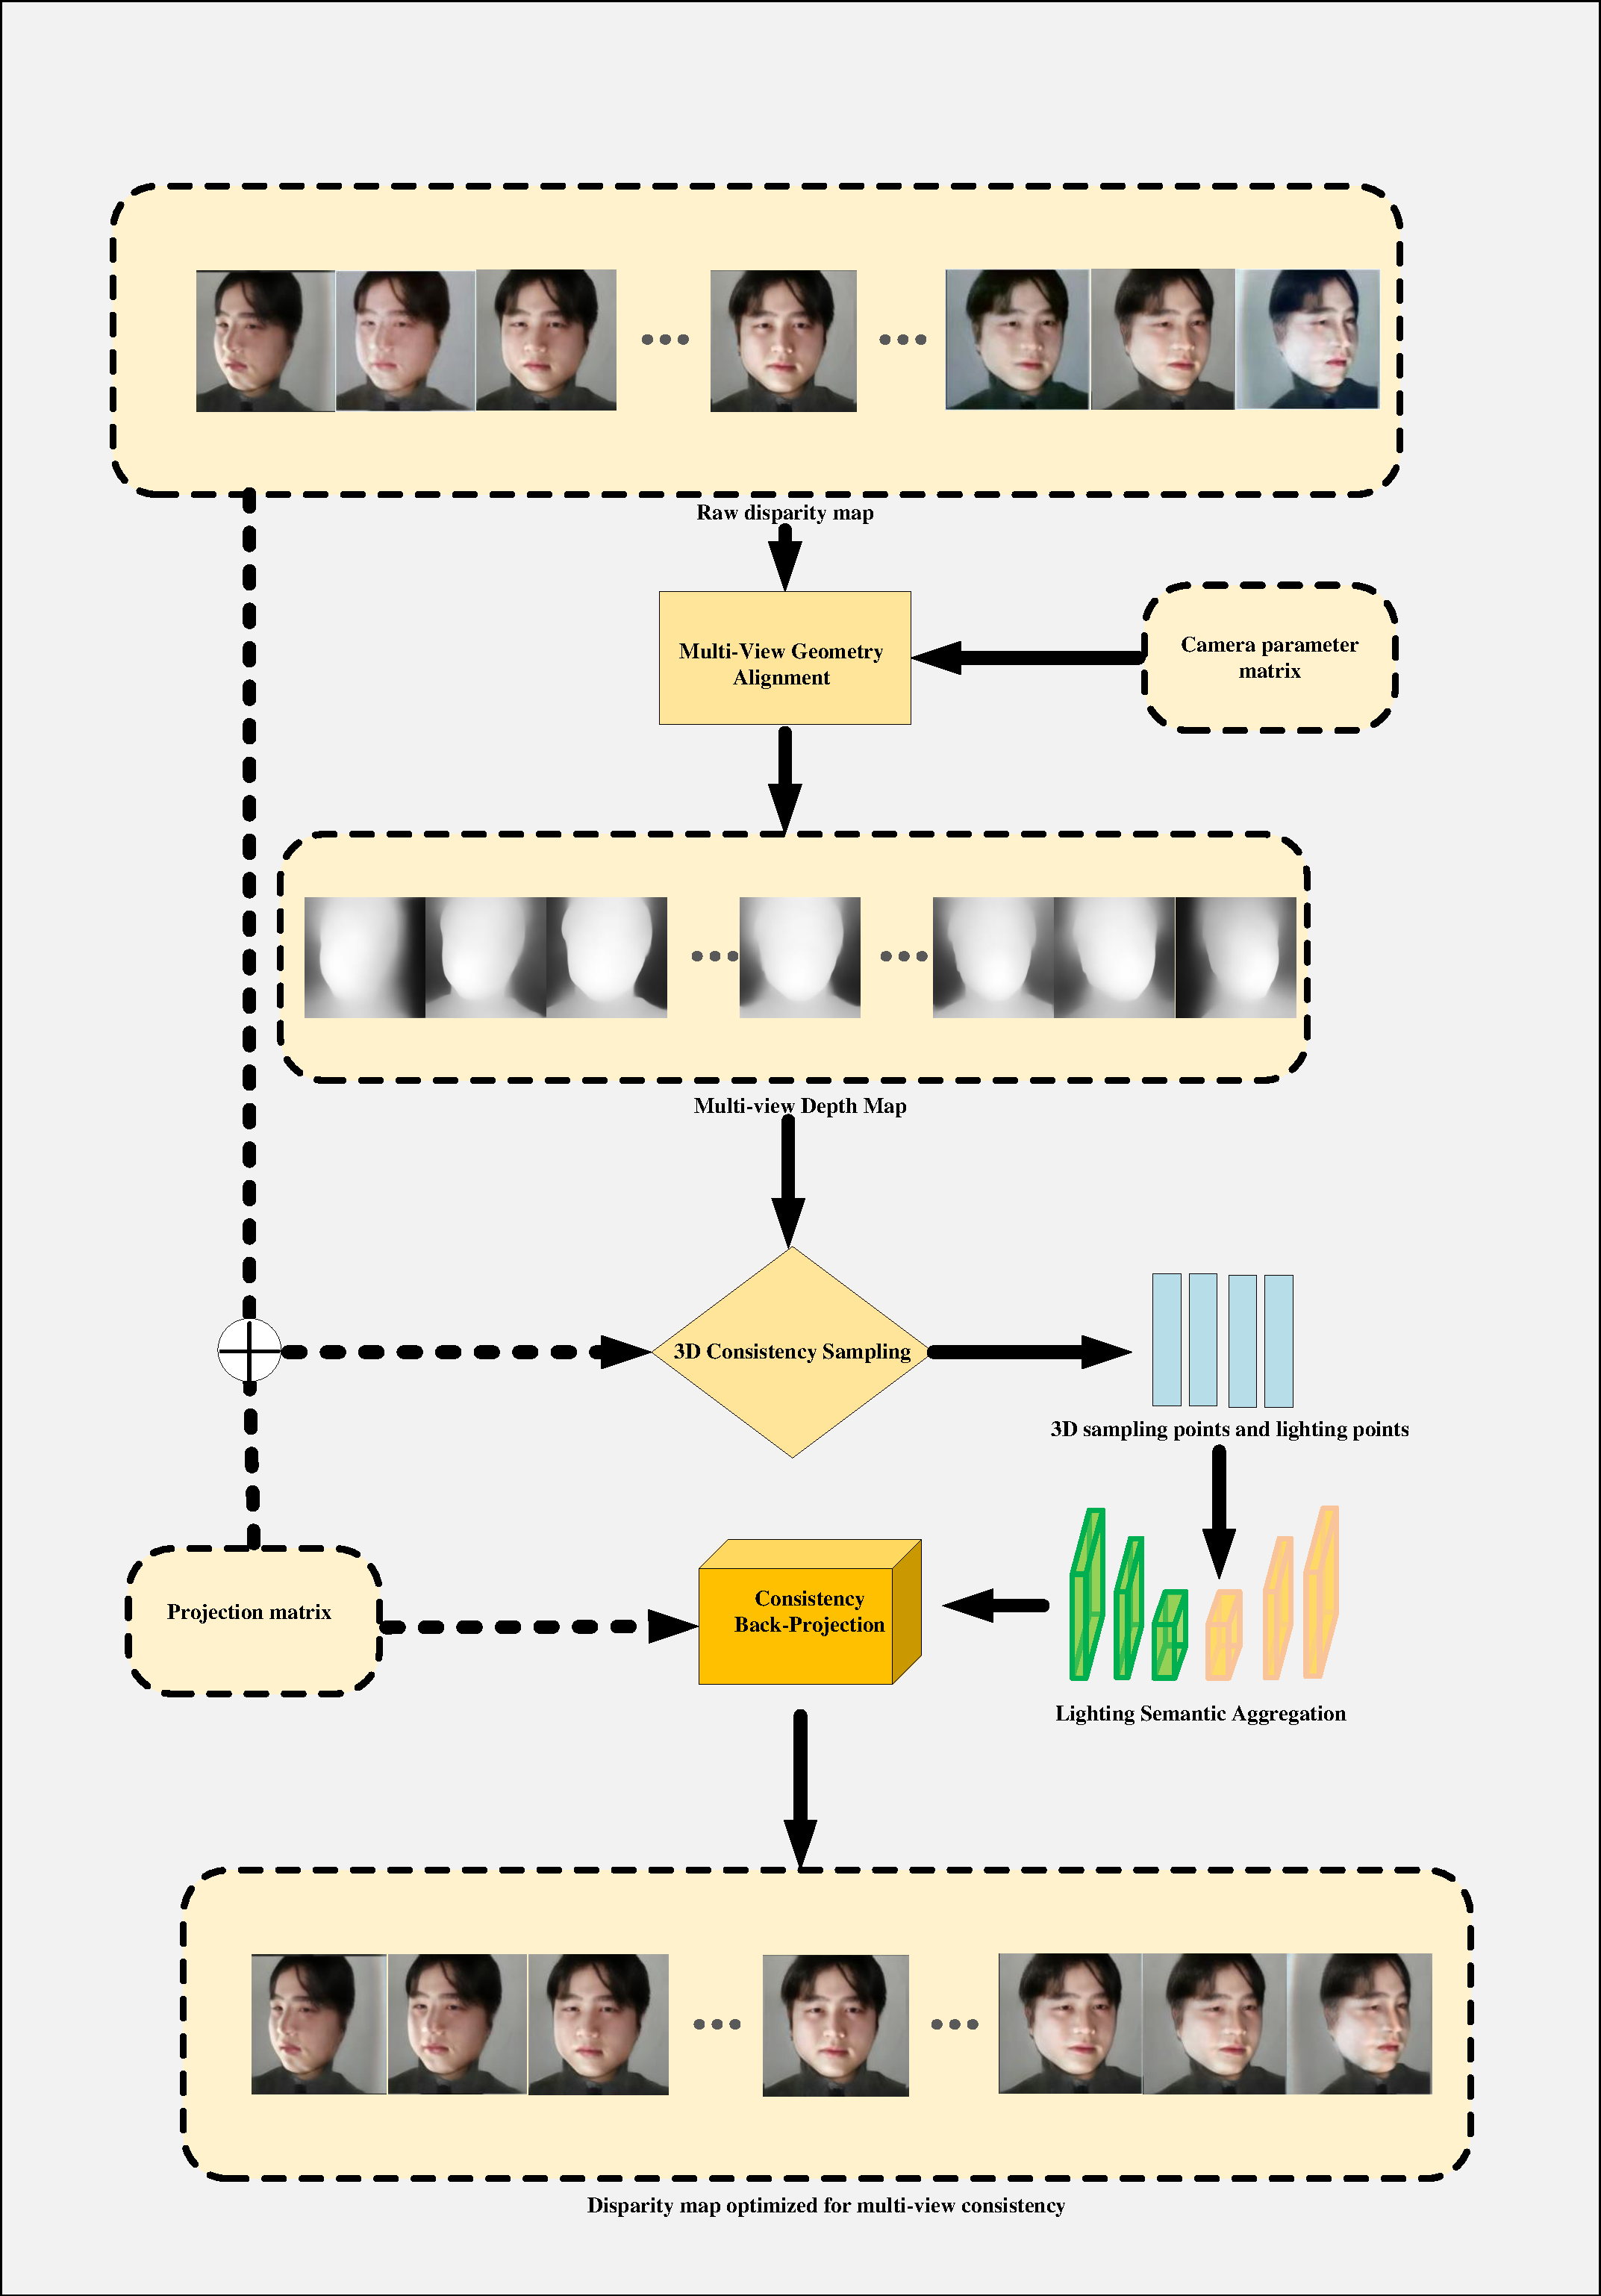
\includegraphics[width=0.9\textwidth,height=20cm]{resources/4p/4-3.pdf}
  % \bicaption{中文标题}{English Caption} % 使用中英文标题
  \caption{多视角一致性优化流程图} % 只使用中文标题
  \label{fig:4-3}
  %\vspace{1 cm} % 使用该指令调整上下间距
\end{figure}

多视角不一致问题的根源在于：光照估计在不同视角之间缺乏统一的三维物理约束。传统图像级方法通常在二维像素空间直接比较颜色差异或特征距离，这类方法忽略了视差变化与遮挡关系的存在，容易导致错误匹配与过度平滑，尤其在人脸边缘、鼻梁高光以及发丝区域问题尤为明显。因此，仅依赖二维空间进行一致性约束难以满足三维光场显示对物理合理性与几何连续性的双重需求。
基于上述问题，本章在时序一致性优化模块的基础上，引入多视角一致性优化模块，通过几何对齐、三维一致性采样、光照语义聚合与一致性回投影四个阶段，将多视角光照统一问题从二维图像域提升至三维空间语义域，实现空间层面的物理一致性约束。在保证各视角合理视差差异存在的前提下，使光照响应在空间维度上保持连续与统一，从而显著增强三维真实感与立体稳定性。
具体流程图如\ref{fig:4-3}所示。

首先将多视图进行多视角几何对齐，该阶段的核心目标在于建立不同视角之间的空间对应关系，使各视角图像能够在统一三维坐标系下进行光照一致性约束。设多视角重光照图像集合为 \(I = \{I_1, I_2, \dots, I_N\}\)，其中 \(N\) 表示视角数量。对于每个视角，系统读取其相机内参矩阵 \(K\) 与外参矩阵 \((R, T)\)，构建对应的投影矩阵 \(\Pi\)。结合已有 NeRF 或多视图深度估计结果，获得统一三维几何模型 \(M\) 或深度图集合 \(D\)。将原本独立的多视角图像映射至同一几何空间，使光照约束具备物理参照系。

与传统基于光流或特征匹配的二维对齐方法相比，几何对齐能够天然处理大视差与遮挡区域问题，避免跨视角误匹配现象，同时为后续三维一致性采样提供稳定基础。

目的是建立不同视角之间的空间对应关系，使各视角图像能够在统一三维空间中进行光照约束，设多视角重光照图像集合为：
\begin{equation}
I = \{I_1, I_2, \dots, I_{90}\}
\end{equation}

其中 \(N\) 为视角数量，对于每个视角，系统读取其相机内参矩阵 \(K\) 和外参矩阵 \((R, T)\)，构建投影矩阵：
\begin{equation}
P_i = K_i [R_i | T_i]
\end{equation}

在完成几何对齐后，本方法并未直接在二维像素空间进行颜色一致性比较，而是将一致性约束提升至三维表面空间。传统多视角方法多采用像素差分策略，容易受到视角角度变化与遮挡关系干扰，导致高光错位或阴影重叠问题。
通过在三维模型 \(M\) 表面均匀采样 \(K\) 个点，将多视角图像统一转化为同一三维点的多次光照观测问题。对于每个采样点，通过投影矩阵将其映射至各视角图像平面，并在对应位置获取光照响应值，从而形成多视角光照观测集合。该设计的核心优势在于：避免二维像素错配。


传统多视角方法多在二维像素空间直接比较颜色差异，容易受遮挡与角度变化干扰。所以将一致性约束提升至三维空间，通过表面采样方式将多视角图像转化为“同一三维点的多次光照观测问题”。

在三维模型 \(M\) 表面均匀采样 \(K\) 个点：
\begin{equation}
P = \{P_1, P_2, \dots, P_K\}
\end{equation}

对于每个采样点 \(P_k\)，通过投影矩阵 \(P_i\) 将其映射至第 \(i\) 个视角图像平面：
\begin{equation}
(u_k^i, v_k^i) = P_i \cdot P_k
\end{equation}

随后在图像 \(I_i\) 中获取该位置的光照响应值：
\begin{equation}
L_k^i = I_i(u_k^i, v_k^i)
\end{equation}

最终每个三维点将获得一组多视角光照观测集合：
\begin{equation}
L_k = \{L_k^1, L_k^2, \dots, L_k^N\}
\end{equation}

该集合表征“同一脸部空间位置在不同视角下的光照估计结果”。

随后进行光照语义聚合（Lighting Semantic Aggregation），由于不同视角可能存在遮挡、高光饱和或预测误差，若直接对多视角光照值进行算术平均，容易导致面部高光消失或阴影模糊。因此本文提出多因子加权光照语义聚合机制，对每个三维点的多视角观测进行可信度融合。

综合权重由三部分构成：

可见性权重：由深度遮挡判断获得。法线夹角权重：衡量表面法线与视角方向关系。光照置信度权重：由光照预测网络输出。

统一光照值通过加权融合计算得到。该机制的物理意义在于模拟真实世界中光照观测的不确定性，使系统能够自动降低不可靠视角的影响，从而获得更加接近真实光照分布的估计结果。

由于不同视角可能存在遮挡、高光饱和或预测误差，直接平均光照值会导致失真。因此引入多因子加权深度语义聚合机制，对多视角光照观测进行可信度融合。

对每个三维点 \(P_k\)，为其在第 \(i\) 个视角下定义综合权重：
\begin{equation}
w_i = w_i^{\text{vis}} \cdot w_i^{\text{norm}} \cdot w_i^{\text{env}}
\end{equation}
其中，分别代表可见性权重（由深度遮挡判断获得）、法线夹角权重（表示表面法线与视角方向的余弦值）和光照置信度权重（由光照预测网络输出）。

统一光照值计算为：
\begin{equation}
L_k^{\text{syn}} = \frac{\sum_{i=1}^{N} w_i L_k^i}{\sum_{i=1}^{N} w_i}
\end{equation}

通过该加权机制，系统能够自动降低被遮挡或不可靠视角的影响，使光照估计更加接近真实物理分布。

最后进行一致性回投优化（Consistency Back-Projection），在获得统一三维光照点云后，需要将其重新映射回各二维视角图像，实现最终的一致性优化。对每个视角执行投影操作，通过光照更新图完成图像修正。

为避免直接替换带来的边缘断裂与纹理丢失问题，本文在回写阶段引入轻量级局部细化网络，仅对高光边界与阴影过渡区域进行自适应优化，从而在保持纹理细节的同时消除高跳变现象。

该阶段的作用相当于从三维一致性到二维视觉一致性的桥梁，保证算法既具备物理合理性，又满足最终视觉呈现需求。

在获得统一三维光照点云后，需要将其重新映射回各二维视角图像，实现最终的一致性优化。对每个视角 \(i\)，执行回投操作：
\begin{equation}
\tilde{I}_i(u, v) = f(I_i(u, v), \Sigma^{\text{upd}})
\end{equation}
其中 \(f(\cdot)\) 表示光照更新函数。为避免直接替换带来的边缘断裂问题，本文在回写阶段引入轻量级局部细化网络进行平滑修正，仅对高光与阴影过渡区域进行自适应优化，从而保留纹理细节。

最终输出为多视角光照一致优化后的图像集合：
\begin{equation}
I^{\text{final}} = \{I_1^{\text{final}}, I_2^{\text{final}}, \dots, I_N^{\text{final}}\}
\end{equation}

本章多视角一致性优化方法通过三维空间采样与语义加权融合，将多视角光照统一问题转化为三维表面光照估计问题，在保证局部真实感的同时显著提升空间维度的光照一致性与物理合理性，为三维光场人像动态光照编辑提供稳定可靠的空间约束基础。

\section{实验}

\subsection{实验细节}
为全面评估本文所提出的人像视频动态光照编辑方法在真实三维光场显示环境下的实际表现，实验部分同时采用自建数据集展示与公开数据集定量评估相结合的方式开展验证。


在视觉效果展示方面，本文主要基于自建人像视频光场数据集进行实验。该数据集由多视角同步采集设备获取，覆盖多种人脸姿态变化、表情变化及光照方向变化场景，能够充分体现动态光照编辑在真实人像序列中的表现能力。所有展示效果图均来源于三维光场显示设备的真实拍摄结果，而非二维渲染图或离线合成图像，从而更真实地反映动态光照编辑在裸眼三维显示环境中的视觉效果与空间连续性表现。

在定量评估部分，为保证实验的客观性与对比方法之间的公平性，本文选取公开多视角人像数据集进行测试，并在统一分辨率、统一光照参数及统一评测标准下与现有方法进行横向对比。通过在公开数据集上的评测，可以有效避免自建数据集带来的偏置问题，使实验结果具有更强的学术说服力与可重复性。

实验采集场地、光照布置方式以及三维显示终端设备均与论文第三章中所介绍的实验平台保持一致，包括多视角相机阵列布局方式、可控光源阵列配置以及裸眼三维光场显示终端型号，从而保证不同章节实验结果之间的一致性与系统连贯性。所有动态光照编辑结果在三维光场显示设备上进行实时或准实时播放，并通过相机进行实拍记录，以确保评估结果能够真实反映人眼在三维观察环境下的视觉体验。

在实验评价体系方面，本文采用分层量化策略以全面验证方法性能。针对整体图像生成质量，选取感知相似度指标（LPIPS）与身份一致性（ID Consistency）进行评估，分别衡量生成结果的视觉自然度与身份特征保持能力；针对时序一致性，采用光流扭曲误差（Warping Error, WE）、帧间感知距离（Inter-frame LPIPS）、时间光照不一致度（Temporal LI）及光照误差（Lighting Error, LE）重点考核动态序列的帧间过渡平滑性。此外，通过控制变量法设计消融实验，定量分析了各核心模块对最终性能的具体贡献。

\subsection{客观实验及实验分析}
（1）显示质量对比实验

为验证本文方法在引入时间与空间一致性约束后不会对视觉生成质量产生负面影响，本节在动态光照视频条件下对关键帧生成效果进行对比分析。不同于第三章针对静态单帧图像的视觉质量评估，本节重点关注引入时间与空间一致性约束后对视觉质量的影响。

图\ref{fig:4-4}(a)和图\ref{fig:4-4}(b)展示了不同方法在相同光照编辑强度下的关键帧重光照结果。从视觉结果可以观察到，对比方法在高光区域与阴影过渡区域存在局部细节丢失或光照边界模糊现象，而本文方法在保持肤色自然过渡的同时，能够较为稳定地保留面部微表情与细节纹理。该结果表明，引入时序与多视角一致性约束并未对图像清晰度与真实感产生明显退化。

\begin{figure}[htbp]  % [H] 强制当前位置，也可改用 [htbp] 自动排版
    \centering  % 整体居中
    
    % 第一张图片（a）：minipage 占满整行宽度
    \begin{minipage}{\textwidth}
        \centering  % 图片在 minipage 内居中
        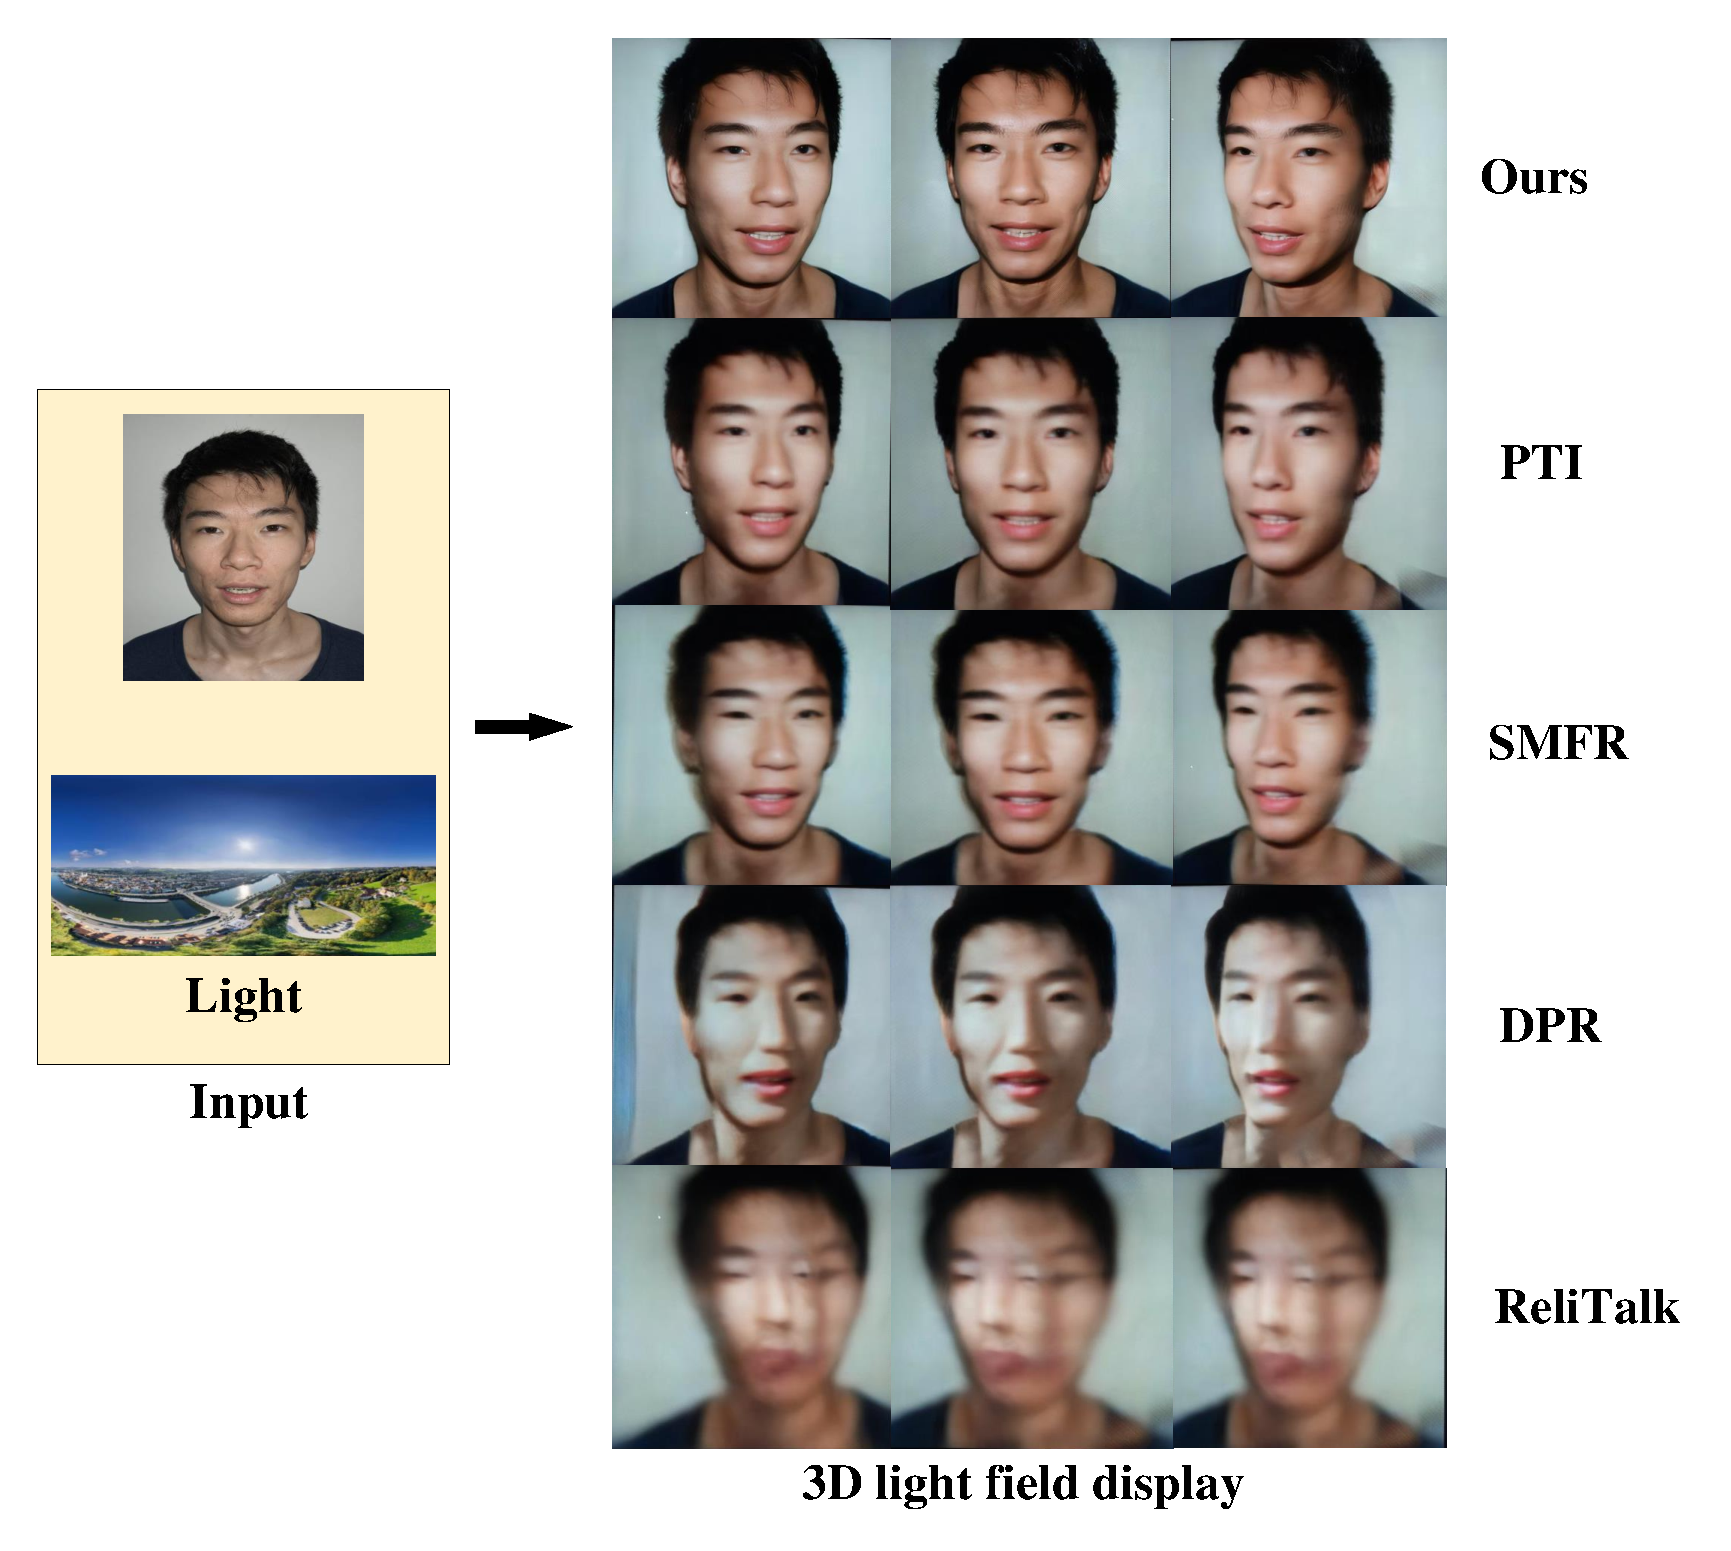
\includegraphics[width=0.8\textwidth]{resources/4p/4-4a.pdf}  % 图片宽度为文本80%
        \caption*{(\textbf{a}) }  % 子图题注（无编号）
        \label{subfig:fig_a}  % 子图引用标签
    \end{minipage}
    
    \vspace{0.5cm}  % 两张图片之间的垂直间距（可调整，如 0.3cm/1em）
    
    % 第二张图片（b）：minipage 占满整行宽度
    \begin{minipage}{\textwidth}
        \centering
        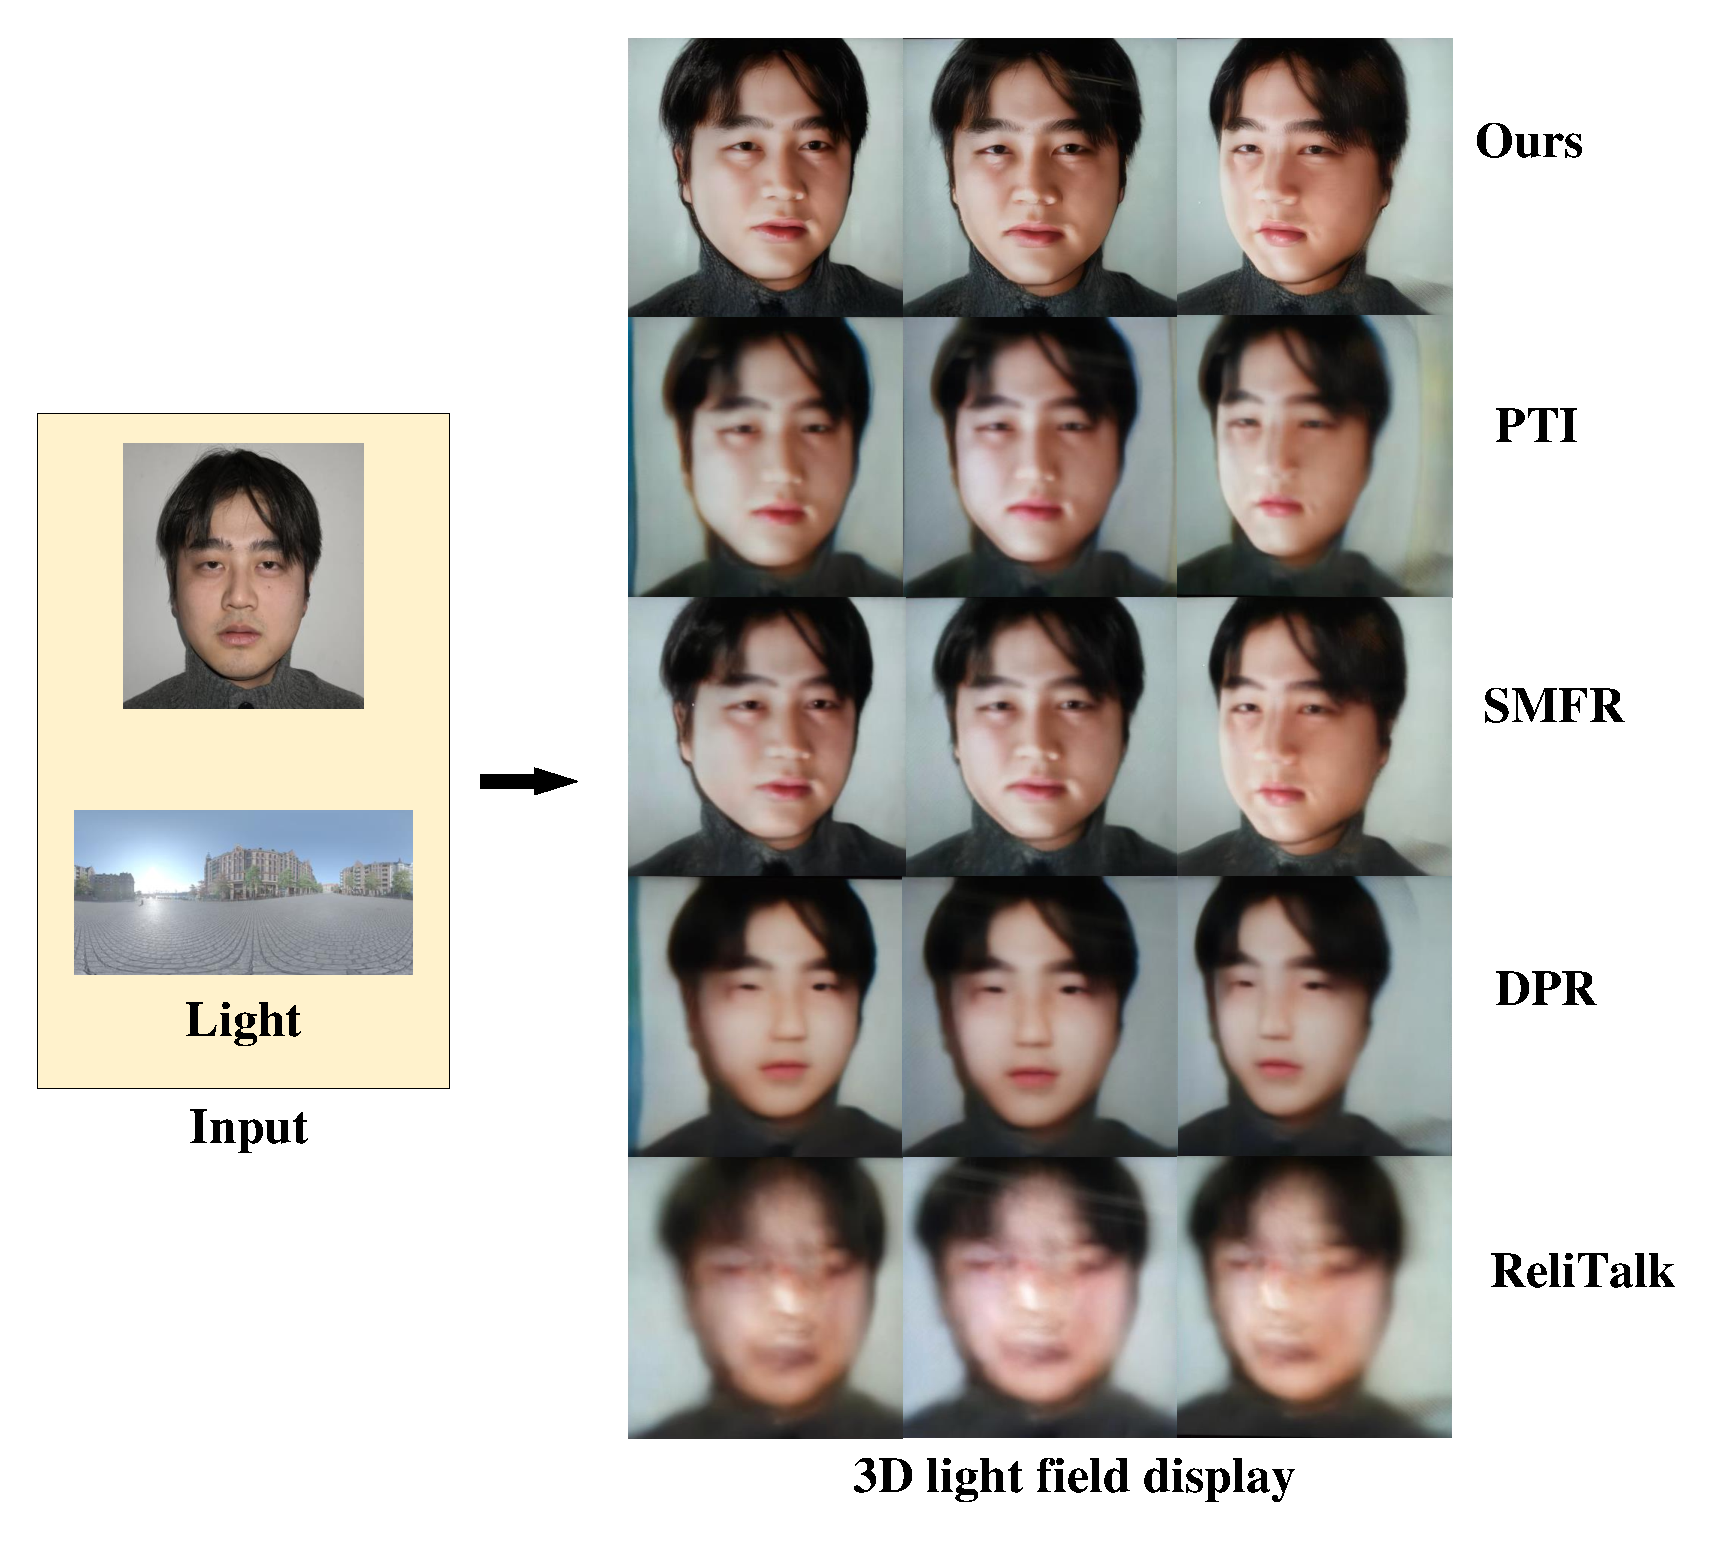
\includegraphics[width=0.8\textwidth]{resources/4p/4-4b.pdf}
        \caption*{(\textbf{b})}
        \label{subfig:fig_b}
    \end{minipage}
    
    % 整张图的总题注（带自动编号）
    \caption{使用不同方法在三维显示器上的显示结果}
    \label{fig:4-4}
\end{figure}

定量结果如表\ref{tab:quantitative_results}所示，本文方法在感知质量指标上与第三章单帧方法保持相当水平，进一步说明一致性优化模块在提升稳定性的同时未引入显著视觉质量损失。

\begin{table}[htbp]
  \centering
  \caption{同一观看视角下与其他方法的指标对比结果}
  \label{tab:quantitative_results}
  \small
  % 调整表格宽度为页面全宽，自动分配列宽
  \begin{tabular*}{\textwidth}{@{\extracolsep{\fill}} lcccc @{}}
  \toprule
  Method & FID $\downarrow$ & PSNR $\uparrow$ & SSIM $\uparrow$ & LPIPS $\downarrow$ \\
  \midrule
  PTI    & 36.4244          & 29.6642         & 0.8188          & 0.2240            \\
  SMFR   & 37.1246          & 25.4346         & 0.7465          & 0.2342            \\
  DPR    & 37.6444          & 24.1121         & 0.6245          & 0.2344            \\
  ReTalk & 40.2454          & 22.4454         & 0.4145          & 0.2855            \\
  Ours   & \textbf{33.5501}          & \textbf{32.0226}         & \textbf{0.8954}          & \textbf{0.1912}            \\
  \bottomrule
  \end{tabular*}
\end{table}



（2）多视角一致性对比实验

\begin{figure}[htbp]  % [H] 强制当前位置，也可改用 [htbp] 自动排版
    \centering  % 整体居中
    
    % 第一张图片（a）：minipage 占满整行宽度
    \begin{minipage}{\textwidth}
        \centering  % 图片在 minipage 内居中
        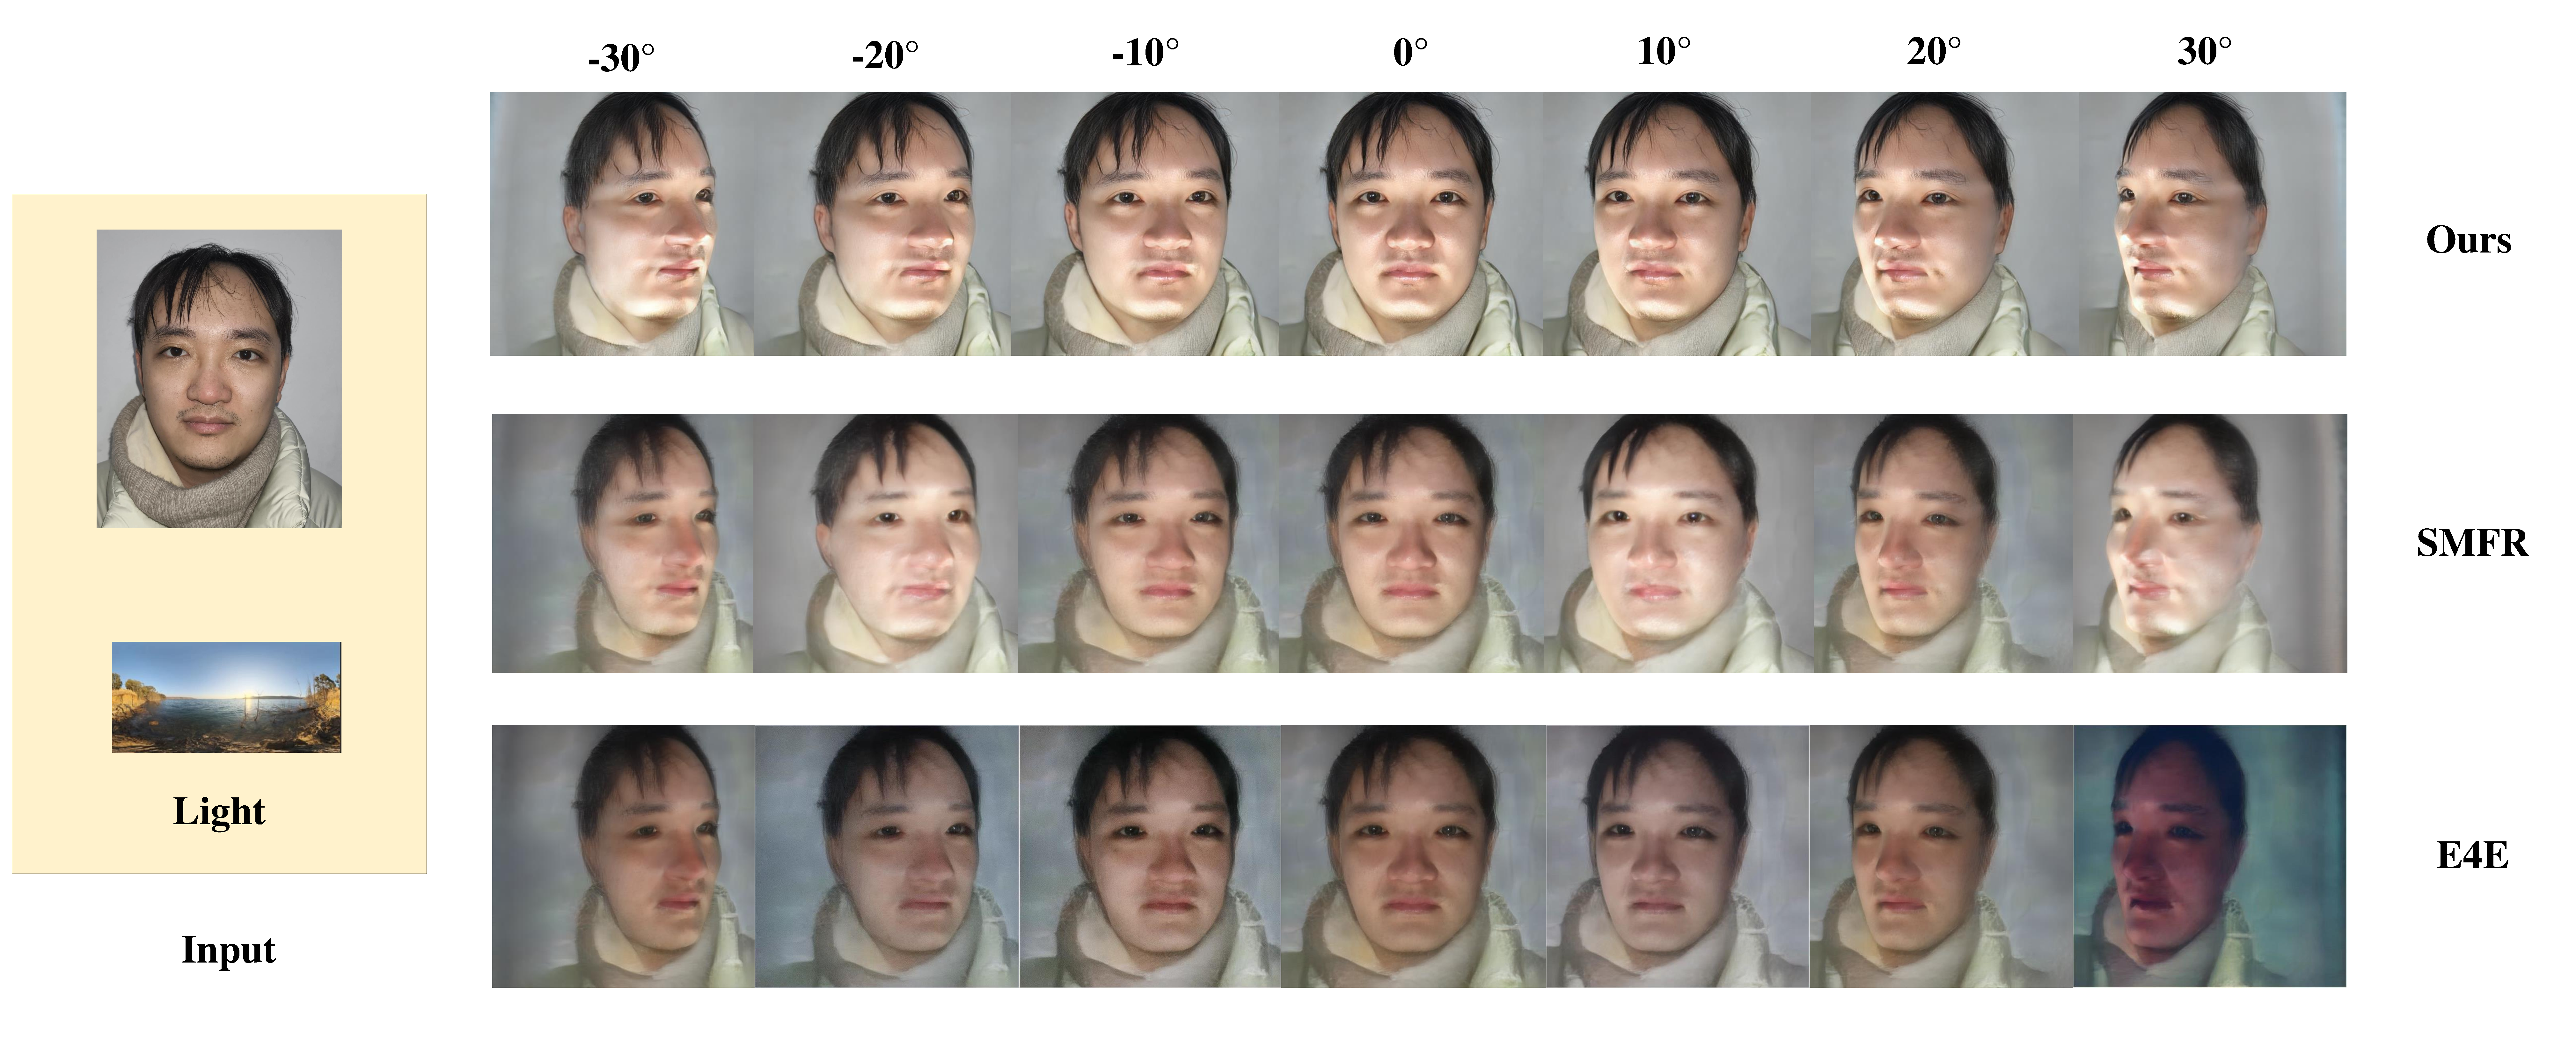
\includegraphics[width=0.9\textwidth,height=5.2cm]{resources/4p/4-5a.pdf}  % 图片宽度为文本80%
        \caption*{(\textbf{a}) }  % 子图题注（无编号）
        \label{subfig:fig_a}  % 子图引用标签
    \end{minipage}
    
    \vspace{0.5cm}  % 两张图片之间的垂直间距（可调整，如 0.3cm/1em）
    
    % 第二张图片（b）：minipage 占满整行宽度
    \begin{minipage}{\textwidth}
        \centering
        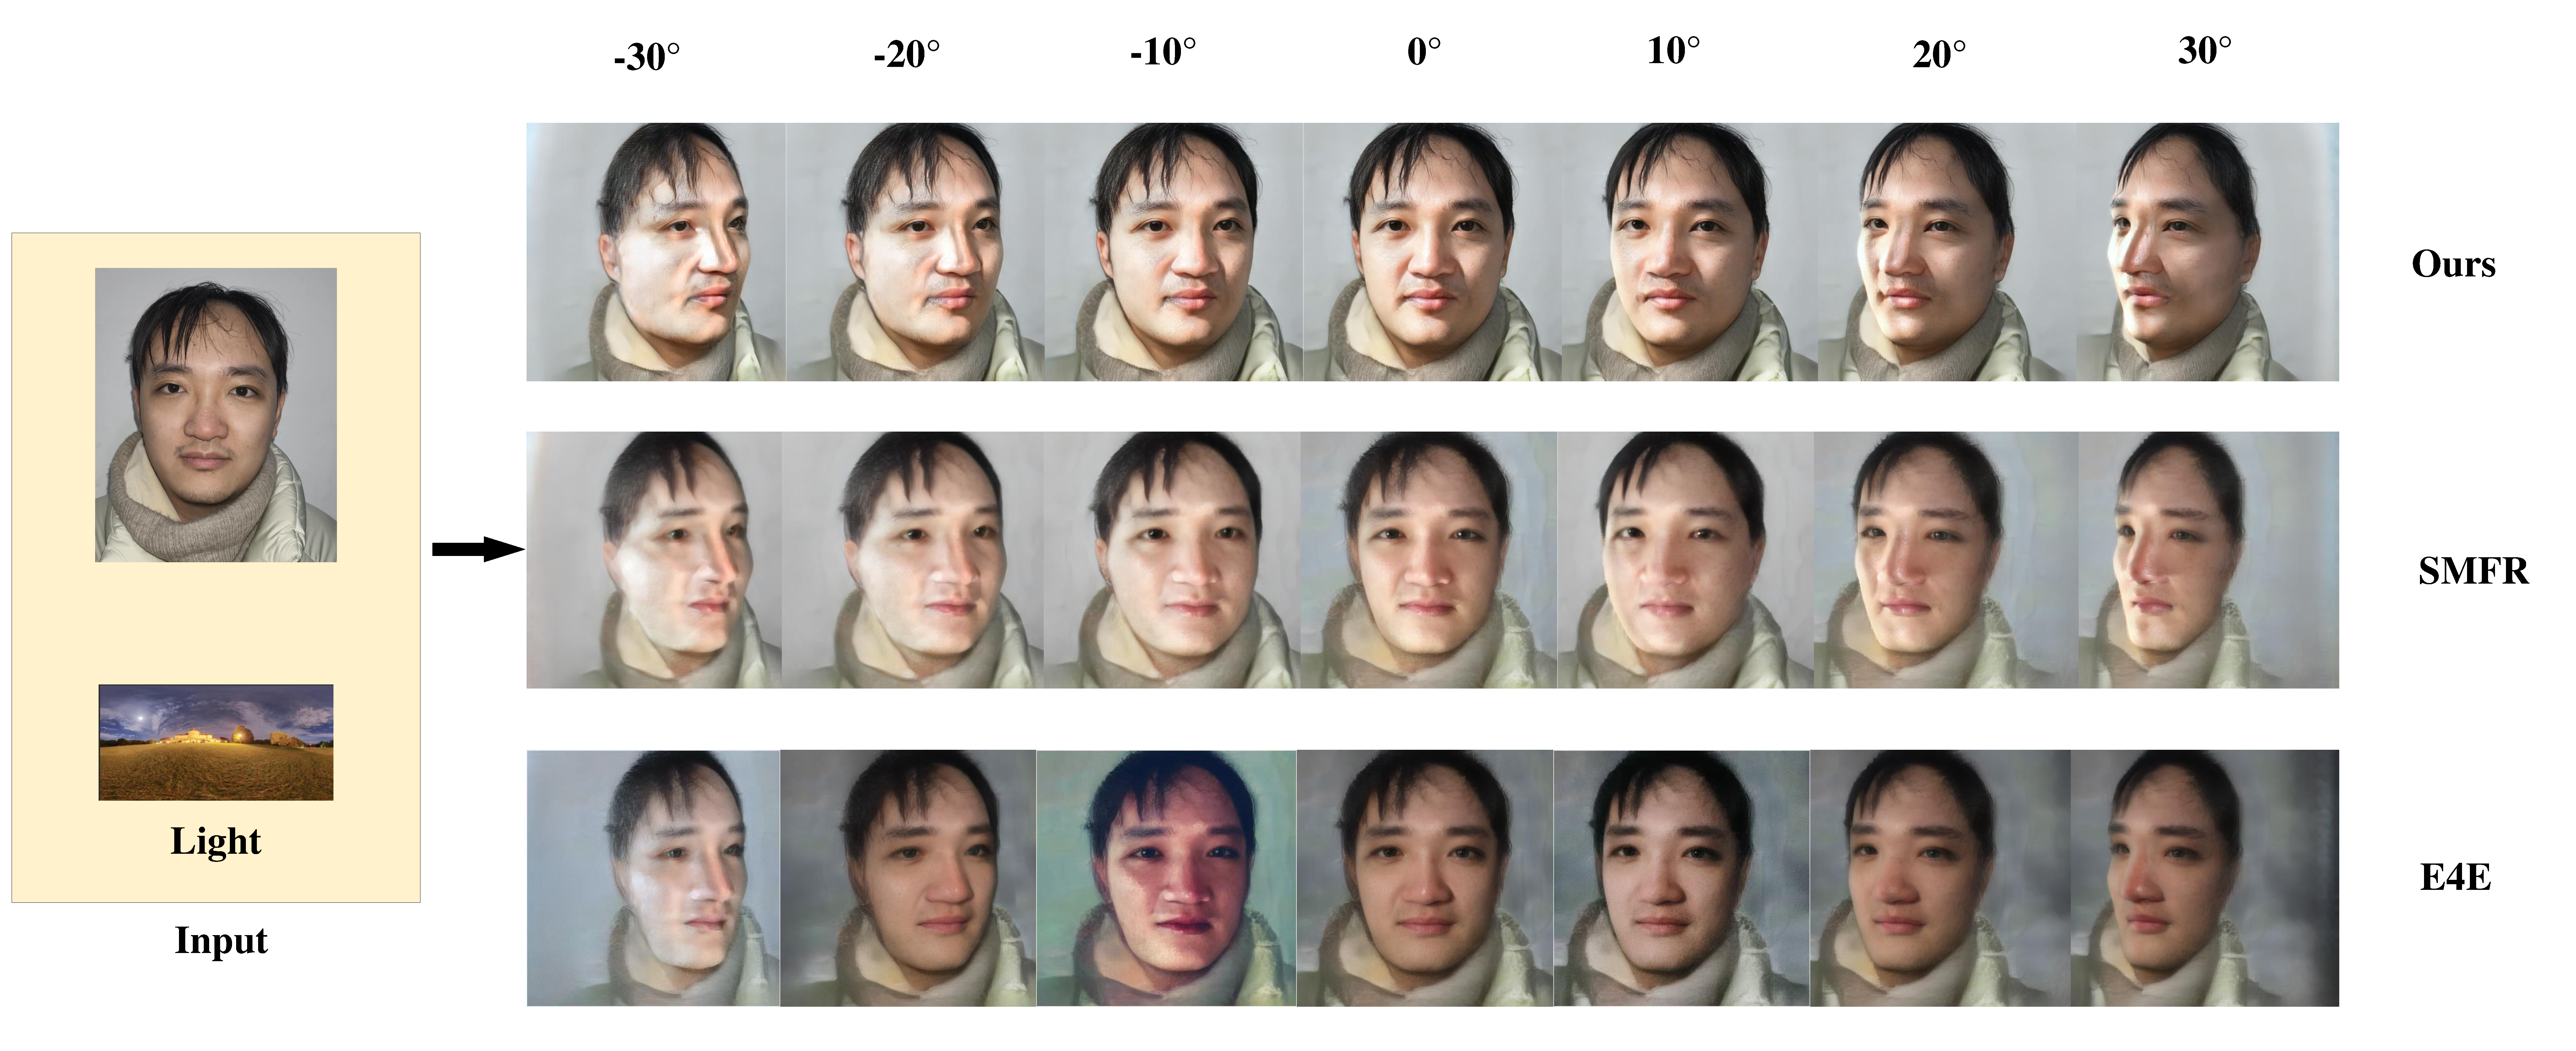
\includegraphics[width=0.9\textwidth,height=5.2cm]{resources/4p/4-5b.pdf}
        \caption*{(\textbf{b})}
        \label{subfig:fig_b}
    \end{minipage}
    
    % 整张图的总题注（带自动编号）
    \caption{不同光照下不同方法的多视角一致性结果对比}
    \label{fig:4-5}
\end{figure}

多视角一致性是三维光场显示中影响立体感的关键因素。若不同视角间的光照响应存在明显差异，将导致观察者在视点切换过程中产生亮度跳变与结构不连贯现象，从而削弱空间真实感。因此，仅依赖单视角重光照质量评估难以全面反映光场显示效果，必须引入跨视角一致性指标进行量化分析。图\ref{fig:4-5}给出了不同方法在多视角条件下的重光照结果对比，可以观察到，对比方法在侧视角区域存在局部光照偏移与阴影方向不统一现象，而本文方法在多视角之间保持了较为一致的高光位置与阴影分布趋势。

\begin{table}[htbp]
  \centering
  \caption{不同方法的多视角光照一致性对比}
  \label{tab:multiview_consistency}
  \begin{tabular}{lccccc}
    \toprule
    Method & $-0.5$ rad & $-0.25$ rad & $0$ rad & $0.25$ rad & $0.5$ rad \\
    \midrule
    SMFR   & 0.4856     & 0.7621      & -       & 0.7738     & 0.5102    \\
    E4E    & 0.6117     & 0.7983      & -       & 0.7895     & 0.6214    \\
    Ours   & \textbf{0.6523} & \textbf{0.8356} & -       & \textbf{0.8414} & \textbf{0.6615} \\
    \bottomrule
  \end{tabular}
\end{table}
我们采用多视角光照一致性（Multi-view Lighting Consistency）作为核心量化指标。该指标用于衡量在同一目标光照条件下，不同视角生成的重光照图像，其光照分布的统一程度与物理合理性。
在具体计算中，我们首先对每个样本在不同光照角度（如 −0.5 rad、−0.25 rad、0.25 rad、0.5 rad）下进行重光照生成，然后使用 ArcFace 模型分别提取原始图像和重光照后图像的人脸特征向量。最后，通过计算这两个特征向量之间的相似度（通常是余弦相似度），得到 Relit Image Identity Similarity 的数值。该指标数值越高，表明多视角下的光照分布越统一，物理合理性越强。

实验结果如表\ref{tab:multiview_consistency}，本文方法在所有光照角度下均取得了最优或次优的一致性得分，显著优于 SMFR 和 E4E 等对比方法，验证了其在多视角光照统一方面的有效性。



（3）时序一致性实验

在视频序列条件下，光照编辑结果若缺乏时间连续性约束，容易产生亮度闪烁与高光抖动等视觉不稳定现象。因此，为验证本文方法在动态人脸视频序列中的时序稳定性，本节从多个维度对时序一致性进行系统评估。
\begin{table}[htbp]
  \centering
  \caption{不同方法的时序一致性指标对比}
  \label{tab:temporal_consistency}
  \begin{tabular}{lcccc}
    \toprule
    Method & ID $\uparrow$ & LE $\downarrow$ & LI $\downarrow$ & WE $\downarrow$ \\
    \midrule
    SMFR   & 37.1246       & 0.8965          & 0.3042          & 0.0022          \\
    E4E    & 37.6444       & 0.8645          & 0.2844          & 0.0007          \\
    Ours   & \textbf{0.5122} & \textbf{0.7922} & \textbf{0.2644} & \textbf{0.0004} \\
    \bottomrule
  \end{tabular}
\end{table}

为进一步验证方法的优越性，我们与 SMFR、E4E 等主流方法进行了定量对比。从定量指标上看：本文方法在所有指标上均取得了最优结果。
光照误差（LE）和光照不一致度（LI）显著降低，证明了光照编辑的准确性和稳定性。光流扭曲误差（WE）降至 0.0004，远低于 SMFR 和 E4E，表明相邻帧之间的空间对齐和光照过渡更加平滑，有效解决了时序闪烁问题。

\begin{figure}[htbp]
  \centering
  %\vspace{1 cm} % 使用该指令调整上下间距
  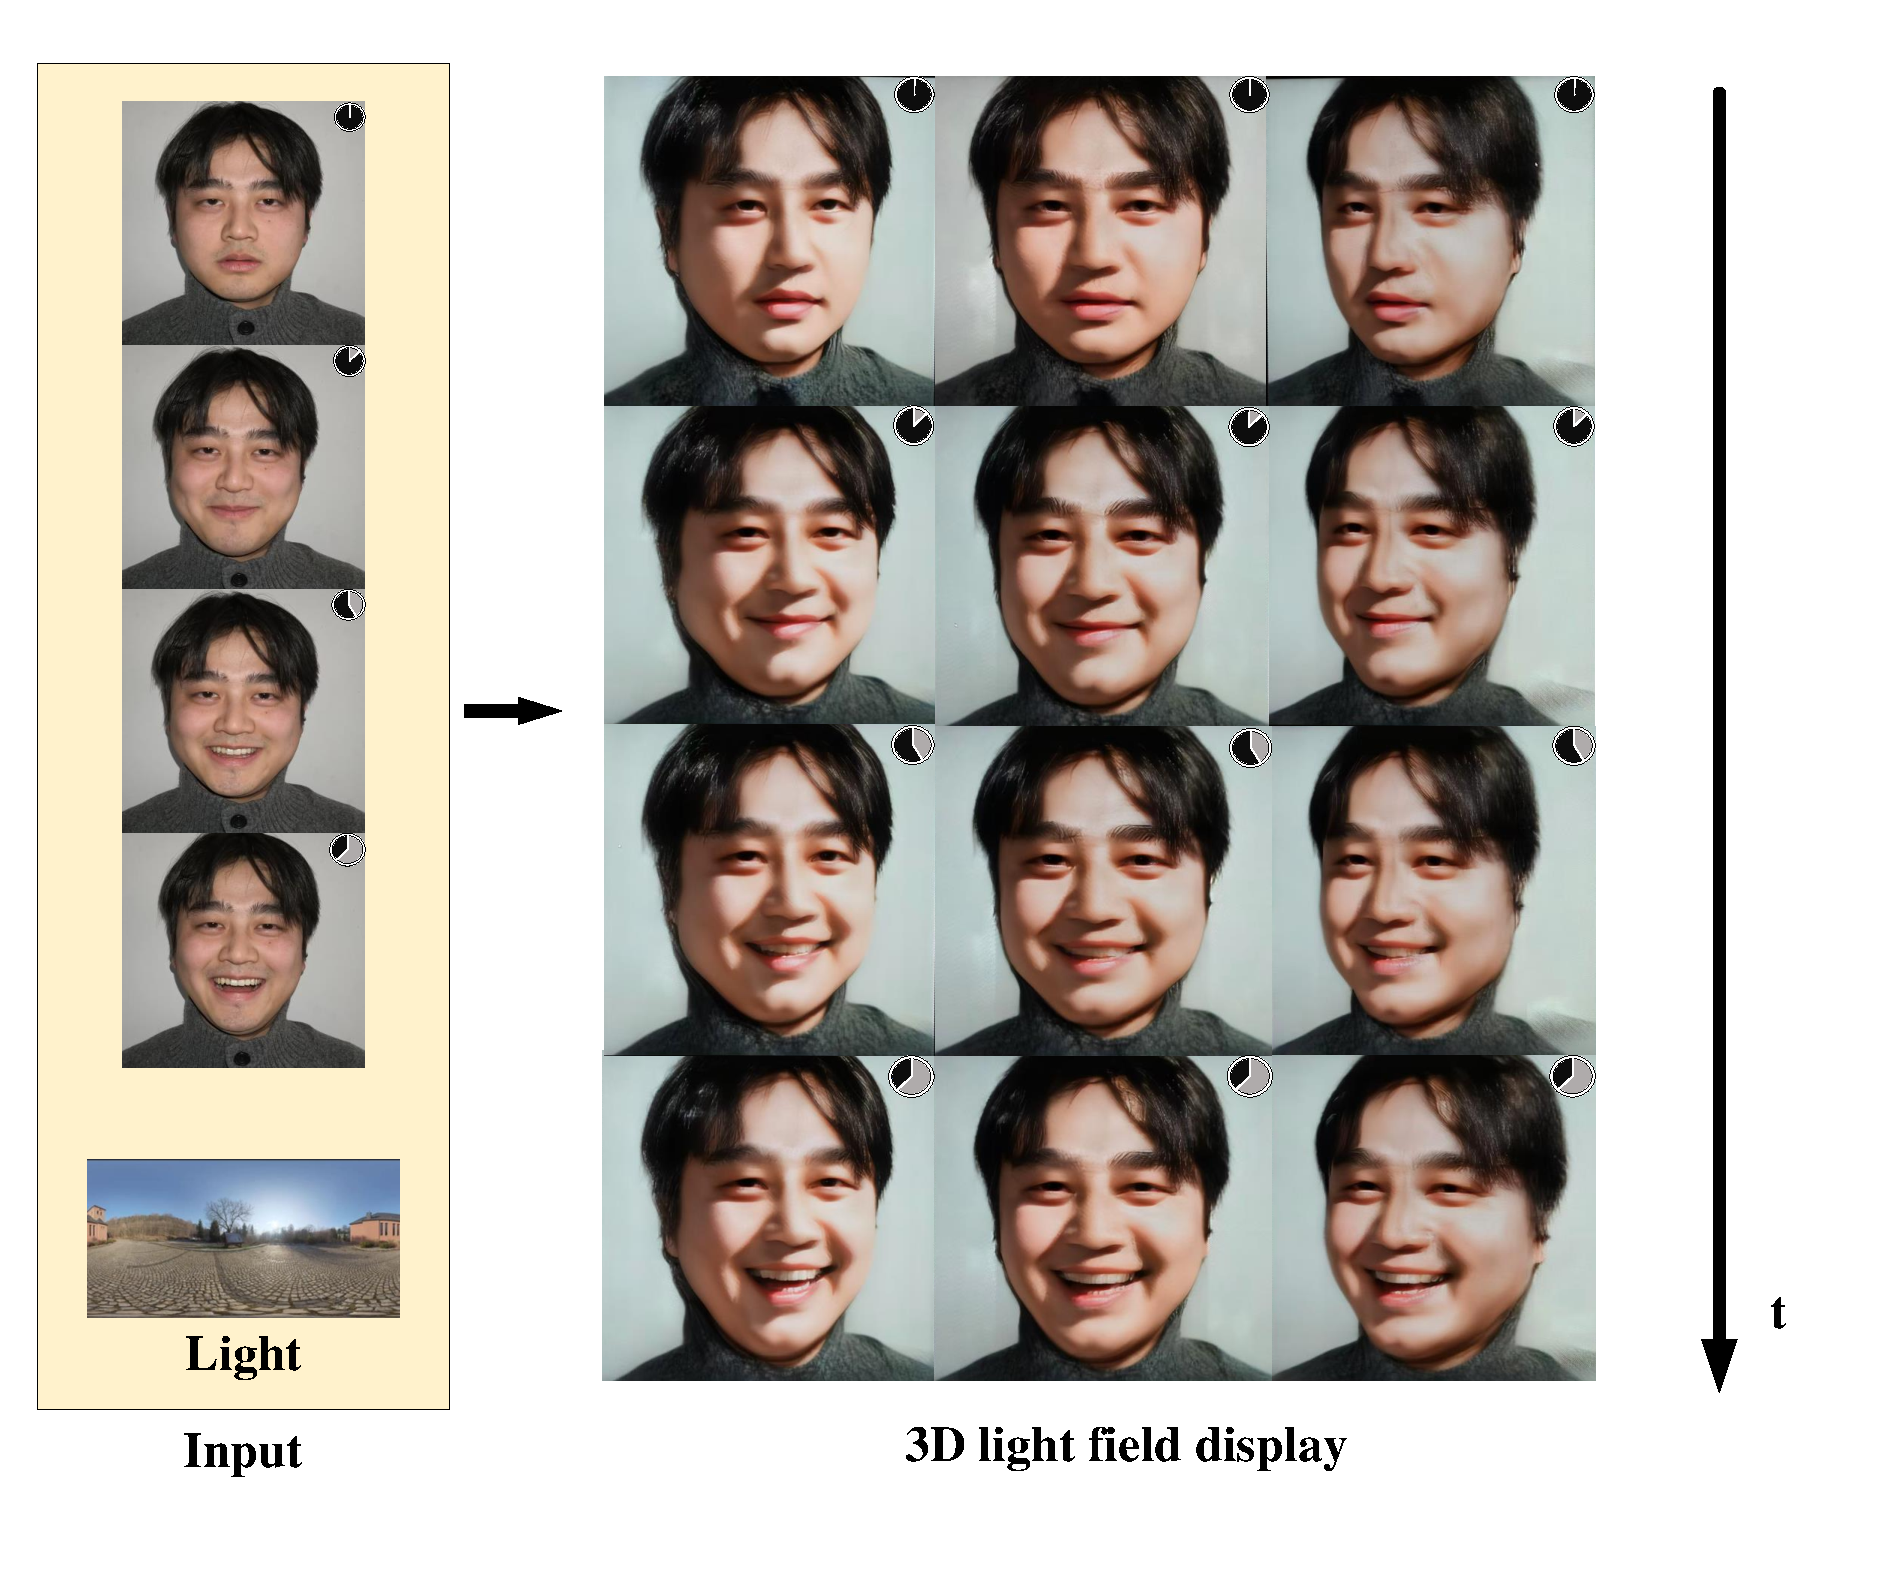
\includegraphics[width=0.9\textwidth,height=10cm]{resources/4p/4-6.pdf}
  % \bicaption{中文标题}{English Caption} % 使用中英文标题
  \caption{} % 只使用中文标题
  \label{fig:4-6}
  %\vspace{1 cm} % 使用该指令调整上下间距
\end{figure}

我们编辑一段包含连续表情变化的人脸视频序列（左侧 “Input” 列），并为其指定一个环境光照（底部 “Light” 图），随后使用本文方法对视频进行重光照处理，生成对应的多视角光场图像（右侧 “3D light field display” 区域）。具体如图\ref{fig:4-6}所示
。从视觉效果上看，本文方法生成的视频序列光照过渡平滑自然，表情和姿态的动态变化与光照实现了解耦，有效抑制了时序闪烁，保证了长序列的视觉一致性，能够满足三维光场显示的应用需求。





\subsection{主观实验及实验分析}
为验证所提方法在实际观看场景中的视觉体验，基于裸眼3D光场显示设备开展主观实验，聚焦动态光照连续性、多视角光照一致性及整体三维沉浸感三大核心维度，对比本文方法与PTI、SMFR、ReliTalk的主观表现。

（1）实验设计

1. 实验条件：沿用第三章硬件平台（单视角分辨率960×540、视场角100°），观测距离2米，20名参与者（男女各10名，视力正常）签署知情同意书。
2. 实验素材：选取6组动态场景（含头部转动、表情变化、光照切换等），包含原始视频及4种方法的编辑结果，均以30fps适配光场显示器。
3. 评价方式：采用5分制评分（1分极差~5分优秀），参与者独立完成评价，场景播放顺序随机化，避免干扰。

（2）实验结果与分析

表\ref{tab:subjective_score}为各方法主观评分平均值，结果表明本文方法在各维度均显著领先，综合评分较PTI提升53.57%。

\begin{table}[htbp]
  \centering
  \caption{主观评分平均值}
  \label{tab:subjective_score}
  \begin{tabular}{lcccc}
    \toprule
    方法       & 动态光照连续性 & 多视角光照一致性 & 整体三维沉浸感 & 综合评分 \\
    \midrule
    PTI        & 3.21           & 2.95             & 3.08           & 3.08     \\
    SMFR       & 2.87           & 2.72             & 2.80           & 2.80     \\
    ReliTalk   & 2.54           & 2.41             & 2.48           & 2.48     \\
    本文方法   & \textbf{4.62}           & \textbf{4.75}             & \textbf{4.81}           & \textbf{4.73}     \\
    \bottomrule
  \end{tabular}
\end{table}

所有参与者认可本文方法光照过渡自然，无闪烁跳变。19名参与者认为跨视角光照无偏移，立体感知更稳定。部分反馈快速头部转动时边缘存在轻微过渡延迟，需后续优化。

（3）实验结论

主观实验证实，本文方法通过时间-空间双维优化，在动态光照连续性、多视角一致性及三维沉浸感上均显著优于对比方法，完全满足裸眼3D光场显示的实际应用需求，主观评价与客观指标结论一致。

\subsection{消融实验}
为验证时序一致性模块（TCN）对整体性能的贡献，我们设计了消融实验：在完整模型中移除时序一致性模块（记为 “w/o TCN”），与完整模型（记为 “Ours”）进行对比，采用光照误差（LE）、光照不一致度（LI）、光流扭曲误差（WE）及身份一致性（ID）四项指标进行评估。
\begin{table}[htbp]
  \centering
  \caption{时序一致性模块消融实验结果}
  \label{tab:ablation_temporal}
  \small
  \begin{tabular*}{\textwidth}{@{\extracolsep{\fill}} lcccc @{}}
  \toprule
    & LE $\downarrow$ & LI $\downarrow$ & WE $\downarrow$ & ID $\downarrow$ \\
  \midrule
  w/o TCN & 0.8544 & 0.2844 & 0.0010 & 0.4322 \\
  Ours    & 0.7811 & 0.2644 & 0.0005 & 0.5122 \\
  \bottomrule
  \end{tabular*}
\end{table}

从表\ref{tab:ablation_temporal}可以看出：移除时序一致性模块后，光照误差（LE）和光照不一致度（LI）明显上升，说明该模块有效提升了光照编辑的准确性与稳定性。光流扭曲误差（WE）从 0.0010 降至 0.0005。身份一致性（ID）从 0.4322 提升至 0.5122，说明该模块在优化时序一致性的同时，并未牺牲身份特征的保持能力，反而通过更稳定的光照过渡，进一步提升了身份一致性。



\section{本章小结}
本章针对静态光照编辑方法扩展至三维光场人像视频时存在的时序闪烁与多视角光照不一致问题，提出了一种时间 - 空间双维联合优化的三维光场人像视频动态光照编辑框架，实现了跨帧光照连续性与跨视角光照统一性的协同提升，弥补了静态方法在动态光场视频场景中的应用缺陷。本章的研究以三维光场显示的实际观看需求为核心，突破了传统视频重光照仅关注二维时序稳定性的局限，将光场数据的 “时间 - 空间双维一致性” 作为核心约束目标，在保证光照编辑可控性的同时，兼顾几何结构稳定与视差连续性，更契合三维光场显示系统的立体观看特性。

为解决时序一致性问题，本章设计了基于特征分离的时序一致性优化模块，采用共享编码网络对相邻帧特征进行提取，保证特征空间分布的一致性；引入光流估计网络实现跨帧特征空间对齐，将时间一致性问题转化为空间对齐问题，避免真实运动被误判为光照闪烁；通过光照分量提取网络实现光照与几何特征的语义解耦，仅对光照响应特征施加时间约束，有效减少了对表情、姿态动态的干扰；同时构建了由特征层 L1 约束与像素层残差 L2 约束组成的双重时序损失函数，既保证光照语义的连续稳定，又抑制像素级的视觉抖动，最后通过轻量级卷积细化网络生成时序一致的重光照结果。针对多视角一致性问题，本章提出了基于三维几何对齐的多视角一致性优化模块，首先通过相机内外参构建投影矩阵，结合 NeRF 或多视图深度估计结果实现多视角图像的三维几何对齐，建立统一的三维物理参照系；随后通过三维模型表面采样，将多视角光照一致性约束从二维像素空间提升至三维表面空间，避免了遮挡、视差带来的误匹配问题；引入多因子加权光照语义聚合机制，结合可见性、法线夹角、光照置信度三重权重对多视角光照观测值进行融合，自动降低不可靠视角的影响；最后通过一致性回投影优化，将统一的三维光照信息映射回各二维视角，并通过局部细化网络修正边缘过渡问题，实现多视角光照的物理一致性表达。

为全面验证方法的有效性，本章从生成质量、多视角一致性、时序一致性及模块贡献度四个方面开展系统实验，结合自建多视角人像视频数据集与公开数据集，采用定性对比与定量分析相结合的方式，与当前主流的人像重光照模型进行公平对比。实验结果表明，本文方法在保证图像生成质量的前提下，在 LI、LE 等多视角一致性指标与 WE、帧间 LPIPS 等时序一致性指标上均取得最优结果，有效解决了多视角光照偏移、帧间光照闪烁等问题。消融实验进一步验证了时序一致性模块的有效性。

本章提出的动态光照一致性优化框架，有效解决了三维光场人像视频光照编辑中的核心问题，提升了动态光场内容的视觉真实感与沉浸感，为三维光场视频的光照编辑提供了新的技术思路。但本方法目前仍聚焦于人像场景，对复杂非人像场景的适应性有待提升，后续可进一步研究几何与光照特征的精细化解耦方法，探索多场景、多物体的三维光场视频动态光照编辑策略，提升算法的通用性与实用性。



